\documentclass[11pt,a4paper]{article}
\usepackage[margin=25mm,headheight=15pt]{geometry}
\usepackage[T1]{fontenc}
\usepackage[utf8]{inputenc}
\IfFileExists{libertinus.sty}{\usepackage{libertinus}}{\usepackage{lmodern}}
\usepackage{microtype,amsmath,amssymb,amsthm,mathtools}
\usepackage{booktabs,tabularx,longtable,array,graphicx}
\usepackage{xcolor,fancyhdr,titlesec,enumitem,listings,xurl}
\usepackage[colorlinks=true,linkcolor=blue!45!black,citecolor=blue!45!black,urlcolor=blue!45!black]{hyperref}
\hypersetup{pdftitle={Exact Boundary Corrections for Thue--Morse Diffraction},pdfauthor={Research article prepared with OpenAI ChatGPT for Vladimir Reshetnikov},pdfsubject={Signed Stern polynomials, positive spectral extrapolation, and sharp Sobolev limits}}
\pagestyle{fancy}\fancyhf{}
\fancyhead[L]{\small Thue--Morse boundary corrections}
\fancyhead[R]{\small\thepage}
\renewcommand{\headrulewidth}{0.3pt}
\titleformat{\section}{\Large\bfseries}{\thesection}{0.7em}{}
\titleformat{\subsection}{\large\bfseries}{\thesubsection}{0.7em}{}
\setlength{\emergencystretch}{2em}
\setlength{\parskip}{0.2em}
\setcounter{tocdepth}{2}
\allowdisplaybreaks
\numberwithin{equation}{section}
\newtheorem{theorem}{Theorem}[section]
\newtheorem{lemma}[theorem]{Lemma}
\newtheorem{proposition}[theorem]{Proposition}
\newtheorem{corollary}[theorem]{Corollary}
\theoremstyle{definition}
\newtheorem{definition}[theorem]{Definition}
\newtheorem{example}[theorem]{Example}
\theoremstyle{remark}
\newtheorem{remark}[theorem]{Remark}
\newcommand{\eps}{\varepsilon}
\newcommand{\T}{\mathbb T}
\newcommand{\Z}{\mathbb Z}
\newcommand{\N}{\mathbb N}
\newcommand{\R}{\mathbb R}
\newcommand{\C}{\mathbb C}
\newcommand{\D}{\mathbb D}
\newcommand{\dd}{\,\mathrm d}
\newcommand{\ee}{\mathrm e}
\newcommand{\ii}{\mathrm i}
\newcommand{\muh}{\widehat\mu}
\newcommand{\mt}{\widetilde\mu}
\newcommand{\ft}{\widetilde f}
\newcommand{\Ht}{\widetilde H}
\newcommand{\pair}[2]{\langle #1,#2\rangle}
\newcommand{\norm}[1]{\lVert #1\rVert}
\newcommand{\abs}[1]{\lvert #1\rvert}
\newcommand{\vnu}{\nu_2}
\newcommand{\Ast}{\mathcal A}
\DeclareMathOperator{\supp}{supp}
\DeclareMathOperator{\dist}{dist}
\lstset{basicstyle=\ttfamily\small,columns=fullflexible,breaklines=true,keepspaces=true,showstringspaces=false,frame=single,rulecolor=\color{black!25},xleftmargin=0.4em,xrightmargin=0.4em}

\title{\bfseries Exact Boundary Corrections\\for Thue--Morse Diffraction\\[0.5em]
\large Signed Stern polynomials, positive spectral extrapolation,\\
and sharp Sobolev limits}
\author{Research article prepared for Vladimir Reshetnikov\\
\small Developed with OpenAI ChatGPT}
\date{4 September 2026}

\begin{document}
\maketitle
\begin{abstract}
The finite Thue--Morse diffraction products approach a singular measure, but their
individual Fourier coefficients do not merely have unspecified finite-size errors.
We identify the entire error below the block-length cutoff with one signed Stern
sequence. If $N=2^m$, $\mu_m$ is the normalized squared modulus of the length-$N$
Thue--Morse polynomial, and $\eta(k)=\widehat\mu(k)$ is the limiting autocorrelation,
then, exactly for $0\le k\le N$,
\[
 \widehat\mu_m(k)-\eta(k)=\frac{(-1)^m}{3N}B_k(-2),
 \qquad \sum_{k\ge1}B_k(-2)z^k
 =z\prod_{j\ge0}(1-z^{2^j})^2.
\]
Consequently the positive probability density
$\widetilde\mu_m=(\mu_m+2\mu_{m+1})/3$ reproduces every limiting Fourier coefficient
through $|k|=N$ exactly. We obtain a distributional first correction, a convergent
analytic finite-size expansion governed by two-colored binary partitions, alternating
Poisson-kernel bounds, and sharp convergence rates in every admissible negative
Sobolev space. The raw approximation has a critical logarithmic loss and a saturation
rate $N^{-1}$; the corrected approximation has the bandwidth-optimal rate
$N^{\sigma-s}$, where
$\sigma=\tfrac12\log_2((1+\sqrt{17})/4)$.
An amplitude-parameter extension gives a sharp positivity threshold $a\ge-2/3$.
All these statements are proved. Classical autocorrelation recurrences, Stern
polynomials, and moment exponents are explicitly separated from the candidate-new
finite-size synthesis. Accompanying code performs 19,037 exact rational checks.
\end{abstract}
\tableofcontents
\clearpage

\section{Scope, prior work, and the contribution}
\label{sec:scope}

\subsection{A particular frontier rather than another formula atlas}
The supplied \emph{Thue--Morse Atlas and Frontiers}~\cite{atlas} develops a large
network of digital, algebraic, analytic, and Fabius--Rvachev identities. Its existing
finite autocorrelation recurrences make the following question natural:
\emph{can the complete finite-block defect be isolated, rather than bounded, and
then removed without losing positivity?} This article answers that question on the
dyadic sequence of block lengths. The answer also identifies precisely the topology
in which the isolated defect has a limit.

The object here is a measure on the frequency circle. It is not the compactly
supported Rvachev density, a Fabius spline approximation, or the tail of a sinc
product. The atlas's cumulant corrections and geometric extrapolation for those
objects therefore do not themselves give the results below. What is shared is a
proof strategy: isolate a finite product, identify the defect algebraically, and only
then estimate it in the appropriate function space.

The atlas source was inspected through the repository on 4 September 2026. The
retrieved \texttt{.tex} blob has Git object identifier
\begin{center}\small\texttt{7be75f3bc86f9c6712eec6d7550eaea53716434a}.\end{center}
This is a file-level provenance marker, not a claim that an older commit recorded
inside that document is the current repository commit.

\subsection{What is established background, and what is proposed as new}
The Riesz product and the finite and infinite Fourier recurrences are established
background; Baake and Grimm~\cite{BG} explicitly give these recurrences and the
singular-continuous limit. The polynomial family $B_k(t)$ is the Stern polynomial
family introduced by Klav\v zar, Milutinovi\'c, and Petr~\cite{Stern}. Neither the
family nor its specialization at $t=-2$ is claimed as a new sequence.

The eigenvalue $1+\sqrt{17}$ and the associated correlation-dimension exponent
are also not new. Zaks, Pikovsky, and Kurths~\cite{ZPK} computed the correlation
dimension; Mauduit, Montgomery, and Rivat~\cite{MMR} studied the even moments of
Thue--Morse generating products. The explicit square-correlation sum used below
also appears in the recent work of Coons, Maz\'a\v c, Pincus--Kazmar, and
Stout~\cite{CMPS}. We give short proofs to expose how these known energies control
an additional finite-size object. General correlation background is developed in
Baake and Coons~\cite{BC}.

The results presented as \emph{candidate-new contributions} are the joint package
of the following connections: the exact Stern boundary term for finite diffraction
and forward correlations; its cancellation by a positive two-level product; the
universal non-measure correction with sharp Sobolev convergence and saturation;
the analytic defect factorization and its positive binary-partition coefficients;
and the amplitude family's sharp positivity threshold and corresponding rate
law. Targeted searches and comparison with the supplied atlas did not locate this
package or these exact formulations. This is a bounded literature assessment,
not a certification of worldwide mathematical priority. The theorems themselves
do not depend on a novelty claim.

\begin{center}
\begin{tabularx}{\textwidth}{@{}p{0.27\textwidth}X@{}}
\toprule
Ingredient or conclusion & Status in this article \\
\midrule
Riesz products and autocorrelation recurrences & Classical inputs, rederived to fix all normalizations. \\
Stern polynomials & Known family; used to identify the entire boundary defect. \\
Square-moment exponent & Known value; not advertised as a newly discovered dimension. \\
Positive Fourier-exact correction & Proved finite-size construction; main candidate-new bridge. \\
Sharp Sobolev error regimes & Proved application of exact defects and known-type energy transfer. \\
Analytic defect and partition coefficients & Proved factorization, positivity, and observable bounds. \\
Amplitude extension & Proved exactness, positivity threshold, and fixed-parameter rate theorem. \\
Lean status & Proof architecture only; no new Lean formalization is asserted. \\
\bottomrule
\end{tabularx}
\end{center}

\section{Normalizations and the finite diffraction measures}
\label{sec:setup}

\subsection{The signed sequence and its two product decompositions}
Write $s_2(n)$ for the number of ones in the binary expansion of $n$, and put
\begin{equation}
 \eps_n=(-1)^{s_2(n)},\qquad
 P_m(z)=\sum_{n=0}^{2^m-1}\eps_nz^n,\qquad N=2^m.
 \label{eq:definitions}
\end{equation}
The empty product has value one, so $P_0=1$. Binary concatenation gives
\begin{equation}
 \eps_{2n}=\eps_n,\quad \eps_{2n+1}=-\eps_n,\quad
 P_m(z)=\prod_{j=0}^{m-1}(1-z^{2^j}).
 \label{eq:binary}
\end{equation}
Indeed, choosing the term $-z^{2^j}$ in a subset of the factors records exactly
the one-bits of the exponent. Both useful recursions follow:
\begin{equation}
 P_{m+1}(z)=(1-z)P_m(z^2)=(1-z^N)P_m(z).
 \label{eq:two-product}
\end{equation}
On the open disk $\D$, the infinite product
\begin{equation}
 E(z)=\prod_{j=0}^{\infty}(1-z^{2^j})
     =\sum_{n=0}^{\infty}\eps_nz^n
 \label{eq:E}
\end{equation}
converges locally uniformly and has no zeros. For $|z|\le r<1$,
$\sum_j|z|^{2^j}<\infty$, so the tail product converges to a nonzero value;
no individual factor vanishes in $\D$. Coefficient stabilization identifies the
Taylor coefficients with $\eps_n$.

\subsection{Fourier conventions}
We use $\T=\R/\Z$ and
\begin{equation}
 \widehat u(k)=\pair{u}{\ee^{-2\pi\ii kx}},\qquad k\in\Z.
 \label{eq:fourier}
\end{equation}
For a measure this means integration; for a periodic distribution it means its
usual pairing with a smooth function. All the measures considered here are real
and even, so their Fourier coefficients are real and even. Define
\begin{equation}
 f_m(x)=\frac1N\abs{P_m(\ee^{2\pi\ii x})}^2
       =\prod_{j=0}^{m-1}(1-\cos(2\pi2^jx)),\qquad
 \mu_m=f_m(x)\dd x.
 \label{eq:fm}
\end{equation}
Orthogonality of the exponentials gives $\int f_m=1$. Thus $\mu_m$ is a
probability measure. Its Fourier coefficients are
\begin{equation}
 r_m(k):=\widehat\mu_m(k)
 =\begin{cases}
 \displaystyle\frac1N\sum_{j=0}^{N-k-1}\eps_j\eps_{j+k},&0\le k<N,\\
 0,&k\ge N,
 \end{cases}\qquad r_m(-k)=r_m(k).
 \label{eq:aperiodic}
\end{equation}
In particular, the coefficient at the endpoint $k=N$ is zero. Keeping this
endpoint in later statements will be useful.

\begin{lemma}[Finite Fourier recursion]
\label{lem:finite-rec}
For $m\ge0$ and $r\ge0$,
\begin{equation}
 r_{m+1}(2r)=r_m(r),\qquad
 r_{m+1}(2r+1)=-\frac12\bigl(r_m(r)+r_m(r+1)\bigr).
 \label{eq:finite-rec}
\end{equation}
The initial sequence is $r_0(k)=\mathbf1_{k=0}$.
\end{lemma}
\begin{proof}
Equation~\eqref{eq:two-product} gives
$f_{m+1}(x)=(1-\cos(2\pi x))f_m(2x)$. The Fourier frequencies of $f_m(2x)$
are even. Multiplication by $1-(\ee^{2\pi\ii x}+\ee^{-2\pi\ii x})/2$ leaves
even coefficients unchanged and creates each odd coefficient from its two
neighbors. This is exactly~\eqref{eq:finite-rec}.
\end{proof}

\begin{proposition}[The limiting measure]
\label{prop:limit}
The measures $\mu_m$ converge weakly to a unique probability measure $\mu$.
Writing $\eta(k)=\widehat\mu(k)$ for $k\ge0$, its coefficients satisfy
\begin{align}
 \eta(0)&=1,&\eta(1)&=-\frac13,\label{eq:eta-base}\\
 \eta(2r)&=\eta(r),&
 \eta(2r+1)&=-\frac12\bigl(\eta(r)+\eta(r+1)\bigr).
 \label{eq:eta-rec}
\end{align}
They are rational and obey $|\eta(k)|\le1/3$ for $k\ge1$.
\end{proposition}
\begin{proof}
The recursion at $k=1$ is
$r_{m+1}(1)=-(1+r_m(1))/2$, whence
\begin{equation}
 r_m(1)=-\frac13+\frac13\left(-\frac12\right)^m.
 \label{eq:mode-one}
\end{equation}
For every $k\ge2$, the right sides in~\eqref{eq:finite-rec} involve smaller
nonnegative indices. Induction on $k$ therefore proves convergence of every fixed
coefficient, with limits~\eqref{eq:eta-base}--\eqref{eq:eta-rec}. Probabilities
on the compact circle have weakly convergent subsequences. Every subsequential
limit has these same Fourier coefficients. Trigonometric polynomials are uniformly
dense in continuous functions, so those coefficients determine the limit uniquely
and the entire sequence converges. Rationality and the bound follow by induction:
for $k\ge2$ each recursion either copies one previously bounded coefficient or
takes minus the average of two such coefficients.
\end{proof}
The measure $\mu$ is the classical singular-continuous Thue--Morse diffraction
measure~\cite{BG}. The results below require the elementary characterization
just proved; singular continuity is only used when contrasting weak convergence
with total-variation convergence.

\section{The signed Stern sequence hidden in the boundary}
\label{sec:stern}

\begin{definition}
Set $g(0)=0$, and for $k\ge1$ set
\begin{equation}
 g(k)=\sum_{j=0}^{k-1}\eps_j\eps_{k-1-j}.
 \label{eq:g-convolution}
\end{equation}
\end{definition}
The shift by one makes the binary recursion particularly simple. Ordinary
convolution of the series~\eqref{eq:E} gives
\begin{equation}
 Q(z):=\sum_{k\ge1}g(k)z^k=zE(z)^2.
 \label{eq:Q}
\end{equation}

\begin{lemma}[Stern recursion and bounds]
\label{lem:stern}
The sequence in~\eqref{eq:g-convolution} satisfies
\begin{equation}
 g(1)=1,\qquad g(2r)=-2g(r),\qquad
 g(2r+1)=g(r)+g(r+1).
 \label{eq:g-rec}
\end{equation}
The last recursion is an identity at $r=0$ and a descending computation for
$r\ge1$. Moreover, for $k\ge1$,
\begin{equation}
 |g(k)|\le k,\qquad g(2^j)=(-2)^j,\qquad
 \vnu(g(k))=\vnu(k).
 \label{eq:g-arithmetic}
\end{equation}
Here $\vnu$ of a nonzero negative integer means the valuation of its absolute value.
\end{lemma}
\begin{proof}
Let $c_n=\sum_{j=0}^n\eps_j\eps_{n-j}$, so $g(k)=c_{k-1}$.
For an odd index $2r-1$, each term has one even and one odd subscript. Splitting
by parity yields $c_{2r-1}=-2c_{r-1}$. For an even index $2r$, the even-even
terms sum to $c_r$, and the odd-odd terms sum to $c_{r-1}$ (with $c_{-1}=0$).
Thus $c_{2r}=c_r+c_{r-1}$, proving~\eqref{eq:g-rec}.

The bound follows because~\eqref{eq:g-convolution} is a sum of $k$ signs.
Iteration of the even recursion proves the power-of-two value. To prove the
valuation statement, first show $g(k)\equiv k\pmod2$ by induction: even indices
give an even value, while at an odd index the two smaller adjacent indices have
opposite parity. Hence every odd-index value is odd. Writing $k=2^ju$ with $u$
odd now gives $g(k)=(-2)^jg(u)$ and the exact valuation.
\end{proof}

The Stern polynomials~\cite{Stern} are defined by $B_0(t)=0$, $B_1(t)=1$,
$B_{2r}(t)=tB_r(t)$, and $B_{2r+1}(t)=B_r(t)+B_{r+1}(t)$. Therefore
\begin{equation}
 g(k)=B_k(-2).
 \label{eq:Stern-identification}
\end{equation}
A useful binary evaluation scheme keeps two adjacent values. For
$v(k)=(g(k),g(k+1))^{\mathsf T}$,
\begin{equation}
 v(2k)=
 \begin{pmatrix}-2&0\\1&1\end{pmatrix}v(k),\qquad
 v(2k+1)=
 \begin{pmatrix}1&1\\0&-2\end{pmatrix}v(k),\qquad
 v(0)=\binom01.
 \label{eq:binary-matrices}
\end{equation}
Thus a single value can be computed using a number of small matrix updates
linear in the bit length of $k$.

\begin{center}\small
\begin{tabular}{@{}r*{8}{r}@{}}
\toprule
$k$ & 1&2&3&4&5&6&7&8\\
$g(k)$ &1&$-2$&$-1$&4&$-3$&2&3&$-8$\\
$3\eta(k)$ &$-1$&$-1$&1&$-1$&0&1&0&$-1$\\
\midrule
$k$ &9&10&11&12&13&14&15&16\\
$g(k)$ &1&6&$-1$&$-4$&5&$-6$&$-5$&16\\
$3\eta(k)$ &$1/2$&0&$-1/2$&1&$-1/2$&0&$1/2$&$-1$\\
\bottomrule
\end{tabular}
\end{center}

\section{An exact finite-block error, including the endpoint}
\label{sec:boundary}

\begin{theorem}[Exact Stern boundary correction]
\label{thm:boundary}
For $m\ge0$, $N=2^m$, and $0\le k\le N$,
\begin{equation}
 \boxed{\quad r_m(k)=\eta(k)+\frac{(-1)^m}{3N}g(k).\quad}
 \label{eq:main-boundary}
\end{equation}
In particular,
\begin{equation}
 |r_m(k)-\eta(k)|\le\frac{k}{3N},
 \label{eq:sharp-mode-bound}
\end{equation}
with equality whenever $k$ is a power of two in this interval.
\end{theorem}
\begin{proof}
At $m=0$, the only indices are $0$ and $1$. Their identities are respectively
$1=1$ and $0=-1/3+1/3$. Suppose the theorem holds at level $m$.
For an even index $2r\le2N$, the difference at the next level equals the old
difference at $r$. Since
\[
 \frac{(-1)^{m+1}}{6N}g(2r)
 =\frac{(-1)^m}{3N}g(r),
\]
the claimed formula follows. For an odd index $2r+1\le2N$, both $r$ and $r+1$
lie in $[0,N]$. Subtracting~\eqref{eq:eta-rec} from~\eqref{eq:finite-rec} gives
\[
 -\frac12\frac{(-1)^m}{3N}\bigl(g(r)+g(r+1)\bigr)
 =\frac{(-1)^{m+1}}{6N}g(2r+1).
\]
This completes the induction, including the zero coefficient at the moving
endpoint. Equation~\eqref{eq:g-arithmetic} proves the bound and its sharpness.
\end{proof}

\begin{corollary}[No nonzero stabilized harmonic is accidentally exact]
For every $k\ge1$ and every $m$ with $2^m\ge k$, $r_m(k)\ne\eta(k)$.
For fixed $k$, the error changes sign with $m$ and has exactly half the magnitude
at the next level. Its rational two-adic valuation is $\vnu(k)-m$.
\end{corollary}
\begin{proof}
Use $g(k)\ne0$ and its valuation in~\eqref{eq:main-boundary}. The denominator
factor $3$ is odd.
\end{proof}

The conclusion is about each fixed coefficient, not uniform convergence on the
entire expanding band: at $k=N$, the error has magnitude $1/3$ for every $m$.
The motion of the cutoff is exactly why function-space estimates later have a
smoothness threshold.

\subsection{Aperiodic versus forward correlations}
The normalized coefficients $r_m$ use a truncated sum, because both indices have
to remain inside the polynomial block. The atlas also considers a forward sum
whose second index may cross the right boundary. Define
\begin{equation}
 C_m(k)=\sum_{j=0}^{N-k-1}\eps_j\eps_{j+k},\qquad
 A_m(k)=\sum_{j=0}^{N-1}\eps_j\eps_{j+k},\qquad 0\le k\le N.
 \label{eq:two-correlations}
\end{equation}
The sum defining $C_m(N)$ is empty.

\begin{theorem}[Both finite-window conventions]
\label{thm:forward}
For $0\le k\le N$,
\begin{align}
 C_m(k)&=N\eta(k)+\frac{(-1)^m}{3}g(k),\label{eq:C-formula}\\
 A_m(k)&=N\eta(k)-\frac{2(-1)^m}{3}g(k).
 \label{eq:A-formula}
\end{align}
\end{theorem}
\begin{proof}
The first formula is Theorem~\ref{thm:boundary} multiplied by $N$.
For the $k$ terms crossing the right boundary, write $j=N-k+r$, $0\le r<k$.
Binary complement inside an $m$-bit block gives
$\eps_{N-1-u}=(-1)^m\eps_u$, and concatenation gives $\eps_{N+r}=-\eps_r$.
Consequently
\[
 A_m(k)-C_m(k)
 =-(-1)^m\sum_{r=0}^{k-1}\eps_{k-1-r}\eps_r
 =-(-1)^mg(k).
\]
Combining the two identities proves~\eqref{eq:A-formula}.
\end{proof}

This theorem upgrades the finite autocorrelation recurrences to a closed
finite-size expression valid simultaneously for every shift through the block
length. In particular, the different constants $1/3$ and $-2/3$ are not conflicting
normalizations: they correspond to distinct window conventions.

\begin{example}[A length-four block]
For $m=2$, the block is $(1,-1,-1,1)$ and
\[
 (r_2(0),\ldots,r_2(4))=(1,-1/4,-1/2,1/4,0).
\]
Subtracting $(\eta(0),\ldots,\eta(4))$ gives
$(0,1,-2,-1,4)/12$, exactly the first five Stern values divided by $3N$.
\end{example}

\section{Positive extrapolation with an exact Fourier band}
\label{sec:positive}

\begin{theorem}[The two-level positive correction]
\label{thm:positive}
For $m\ge0$, define
\begin{equation}
 \mt_m=\frac13\mu_m+\frac23\mu_{m+1}.
 \label{eq:positive-combination}
\end{equation}
It is a probability measure with nonnegative trigonometric-polynomial density
\begin{equation}
 \boxed{\quad
 \ft_m(x)=f_m(x)\left(1-\frac23\cos(2\pi Nx)\right),\quad N=2^m.
 \quad}
 \label{eq:positive-density}
\end{equation}
Its Fourier coefficients satisfy
\begin{equation}
 \widehat{\mt_m}(k)=\eta(k)\qquad (|k|\le N).
 \label{eq:band-exact}
\end{equation}
Among affine combinations $w\mu_m+(1-w)\mu_{m+1}$, it is the unique one agreeing
with the limit at $k=1$. Its density has degree at most $2N-1$.
\end{theorem}
\begin{proof}
The coefficient error at level $m+1$ is $-1/2$ times the error at level $m$
on the common band. The weights $1/3$ and $2/3$ cancel it exactly. The error at
$k=1$ is nonzero; hence any cancelling affine weight must solve
$w-(1-w)/2=0$, which gives $w=1/3$. The second factorization
in~\eqref{eq:two-product} yields
$f_{m+1}=f_m(1-\cos(2\pi Nx))$, proving~\eqref{eq:positive-density}. Its new
factor lies between $1/3$ and $5/3$. Positivity and total mass one also follow
directly from the convex combination. The degree bound is the sum of $N-1$
and $N$.
\end{proof}

For every trigonometric polynomial $\phi$ of degree at most $N$, this gives an
exact integration identity
\begin{equation}
 \int_\T\phi\dd\mu=\int_0^1\phi(x)\ft_m(x)\dd x.
 \label{eq:exact-quadrature}
\end{equation}
Thus a singular measure has a positive, explicitly factored density representing
its entire low-frequency moment vector. This is not an assertion that the two
measures agree on arbitrary sets or arbitrary continuous functions.

\begin{figure}[tb]
\centering
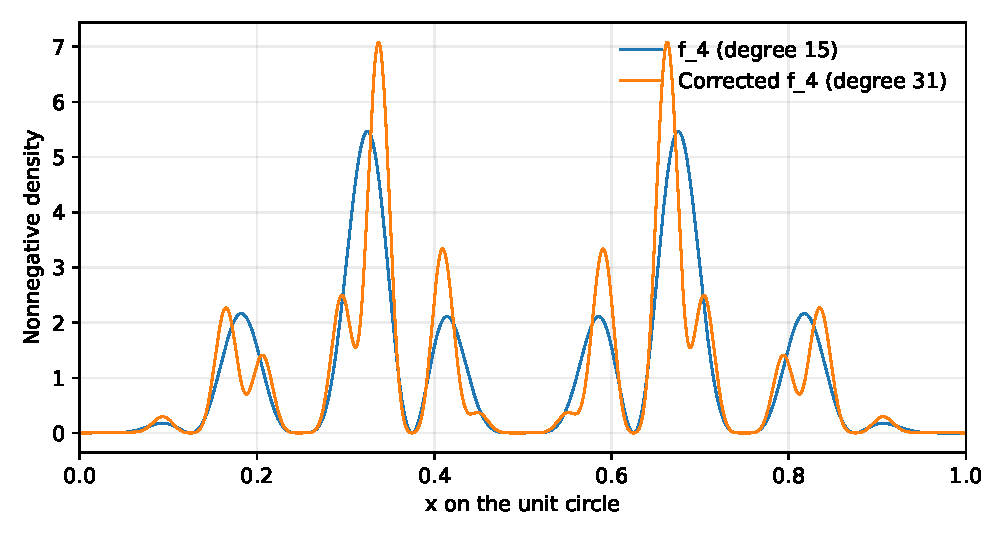
\includegraphics[width=0.94\textwidth]{figures/positive_density.pdf}
\caption{The raw and corrected densities at $m=4$. Both are nonnegative.
The corrected curve reproduces the limiting measure's Fourier coefficients
through $|k|=16$ exactly. The figure makes no assertion of pointwise convergence
to a density of the limit.}
\label{fig:density}
\end{figure}

\subsection{Smooth and analytic observables}
For $r\ge0$, write
\begin{equation}
 \Ast_r(\phi)=\sum_{k\in\Z\setminus\{0\}}|k|^r|\widehat\phi(k)|.
 \label{eq:wiener}
\end{equation}
Every smooth periodic function has finite $\Ast_r$ for every fixed $r$: repeated
integration by parts bounds its Fourier coefficients by any desired power.

\begin{corollary}[Tail-only integration error]
\label{cor:observable}
For an absolutely convergent Fourier series,
\begin{equation}
 \abs{\pair{\mt_m-\mu}{\phi}}
 \le2\sum_{|k|>N}|\widehat\phi(k)|.
 \label{eq:observable-tail}
\end{equation}
Consequently, whenever $\Ast_r(\phi)<\infty$,
\begin{equation}
 \abs{\pair{\mt_m-\mu}{\phi}}\le2N^{-r}\Ast_r(\phi).
 \label{eq:observable-power}
\end{equation}
If $|\widehat\phi(k)|\le M\rho^{|k|}$ for $0<\rho<1$, then
\begin{equation}
 \abs{\pair{\mt_m-\mu}{\phi}}
 \le\frac{4M\rho^{N+1}}{1-\rho}.
 \label{eq:observable-exp}
\end{equation}
\end{corollary}
\begin{proof}
Termwise pairing is justified by absolute convergence and finite total variation.
Every coefficient on the low band vanishes by~\eqref{eq:band-exact}; every other
coefficient of the difference has magnitude at most two because both measures
are probabilities. Summing the Fourier tail gives~\eqref{eq:observable-tail};
comparison with $|k|^r/N^r$ and a geometric series gives the other two statements.
\end{proof}

For a fixed $C^\infty$ observable, the corrected error decays faster than every
power of $N^{-1}$. For a fixed analytic strip it decays exponentially in $N$.
The constants depend on the observable or the strip, so these statements must
not be applied uniformly to probes whose frequencies grow with $N$.

\begin{remark}[Why positivity is a genuine constraint]
Ordinary Richardson extrapolation often uses a negative weight. Here the raw
error alternates in $m$, so the extrapolation weights are both positive. It is
therefore exact on an expanding spectral band without sacrificing the measure
interpretation. This does not imply convergence in total variation: since $\mu$
is singular and each $\mt_m$ is absolutely continuous, their total-variation norm
distance is two, or one under the convention $\sup_A|\mt_m(A)-\mu(A)|$.
\end{remark}

\section{The universal first correction is a distribution, not a measure}
\label{sec:distribution}

\begin{definition}
Let $\nu$ be the real even periodic distribution specified by
\begin{equation}
 \widehat\nu(0)=0,\qquad
 \widehat\nu(k)=\frac13g(|k|)\quad(k\ne0).
 \label{eq:nu}
\end{equation}
\end{definition}
The bound $|g(k)|\le k$ makes this definition legitimate: pairing its Fourier
coefficients with those of a smooth function is absolutely convergent and
continuous in an appropriate smooth seminorm.

\begin{theorem}[One algebraic correction, with a rapidly small weak remainder]
\label{thm:distribution}
There are distributions $R_m$ such that
\begin{equation}
 \mu_m=\mu+\frac{(-1)^m}{N}\nu+R_m,
 \qquad \widehat R_m(k)=0\quad(|k|\le N).
 \label{eq:distribution-expansion}
\end{equation}
For $r\ge1$ and $\Ast_r(\phi)<\infty$,
\begin{equation}
 \abs{\pair{R_m}{\phi}}\le\frac43N^{-r}\Ast_r(\phi).
 \label{eq:R-bound}
\end{equation}
In particular $(-1)^mN(\mu_m-\mu)\to\nu$ in the space of periodic distributions.
The distribution $\nu$ is not a finite signed measure.
\end{theorem}
\begin{proof}
Define $R_m$ by~\eqref{eq:distribution-expansion}. The low coefficients vanish
by Theorem~\ref{thm:boundary}. For $|k|>N$ the finite product has no coefficient,
so
\[
 \widehat R_m(k)=-\eta(|k|)-\frac{(-1)^m}{3N}g(|k|).
\]
Its magnitude is at most $1+|k|/(3N)\le4|k|/(3N)$. Hence
\[
 |\pair{R_m}{\phi}|
 \le\frac4{3N}\sum_{|k|>N}|k||\widehat\phi(k)|
 \le\frac43N^{-r}\Ast_r(\phi),
\]
where $|k|\le N^{1-r}|k|^r$ on this tail. Taking any fixed $r>1$ proves the
renormalized distributional convergence. Finally
$|\widehat\nu(2^j)|=2^j/3\to\infty$. Fourier coefficients of a finite signed
measure are bounded by its total variation, so $\nu$ cannot be one.
\end{proof}

For each fixed smooth observable the expansion has just one nonzero algebraic
finite-size term. All subsequent powers can be assigned zero coefficients, with
a remainder smaller than every prescribed power. This is a weak statement, not
a pointwise expansion of $f_m$. The negative Sobolev spaces in
Section~\ref{sec:sobolev} quantify exactly how much smoothness is required to
promote it to norm convergence.

\section{An exact analytic factorization of all remaining modes}
\label{sec:analytic}

\subsection{The affine Mahler equation and its homogeneous defect}
Define the one-sided Fourier generating functions
\begin{equation}
 H(z)=\sum_{k=0}^{\infty}\eta(k)z^k,\qquad
 H_m(z)=\sum_{k=0}^{N-1}r_m(k)z^k,\qquad |z|<1.
 \label{eq:H}
\end{equation}
These are not the same functions as $E$ and $P_m$: $E$ and $P_m$ encode the
sign sequence, while $H$ and $H_m$ encode autocorrelations.

\begin{lemma}[Affine functional equations]
\label{lem:MahlerH}
Writing $A(z)=1-(z+z^{-1})/2=-(1-z)^2/(2z)$, one has
\begin{equation}
 H(z)=A(z)H(z^2)+\frac1{2z},\qquad
 H_{m+1}(z)=A(z)H_m(z^2)+\frac1{2z}.
 \label{eq:H-Mahler}
\end{equation}
The singularities displayed at zero are removable.
\end{lemma}
\begin{proof}
The even part of either series is the previous series at $z^2$. The odd part is
\[
 -\frac z2\left(H(z^2)+\frac{H(z^2)-1}{z^2}\right)
\]
for the limiting series, and the identical expression with $H_m$ for a finite
one. Adding the even part proves the equations. The constant coefficient is
one on both sides, which also exhibits the cancellation at zero.
\end{proof}

\begin{theorem}[Exact analytic defect]
\label{thm:analytic}
The function
\begin{equation}
 K(w)=\frac{3(1-H(w))}{wE(w)^2},\qquad K(0)=1,
 \label{eq:K}
\end{equation}
is analytic on $\D$. For every $m\ge0$ and $z\in\D$,
\begin{equation}
 \boxed{\quad H_m(z)-H(z)
 =\frac{(-1)^m}{3N}\,zE(z)^2K(z^N).\quad}
 \label{eq:analytic-defect}
\end{equation}
If $\Ht_m=(H_m+2H_{m+1})/3$, then
\begin{equation}
 \Ht_m(z)-H(z)
 =\frac{(-1)^m}{9N}\,zE(z)^2
       \bigl(K(z^N)-K(z^{2N})\bigr).
 \label{eq:analytic-corrected}
\end{equation}
\end{theorem}
\begin{proof}
Subtract the two equations in~\eqref{eq:H-Mahler}. Iterating the resulting
homogeneous equation from $H_0=1$ gives
\begin{align*}
 H_m(z)-H(z)
 &=\left(\prod_{j=0}^{m-1}A(z^{2^j})\right)(1-H(z^N))\\
 &=\frac{(-1)^m}{N}z^{1-N}P_m(z)^2(1-H(z^N)).
\end{align*}
The infinite product splits as $E(z)=P_m(z)E(z^N)$. Substitute
$1-H(w)=wE(w)^2K(w)/3$ to obtain~\eqref{eq:analytic-defect}.
The denominator in~\eqref{eq:K} has no zeros except its explicit first-order
zero at zero, while $1-H(w)=w/3+O(w^2)$, so $K$ is analytic and $K(0)=1$.
Combining two consecutive levels gives~\eqref{eq:analytic-corrected}.
\end{proof}

The proof also supplies a second derivation of the low-band theorem: in
$Q(z)K(z^N)$, the nonconstant terms of $K$ can contribute only from degree $N+1$
onward. The exact boundary correction is precisely the constant term $K(0)=1$.

\subsection{Two-colored binary partitions and positive defect coefficients}
Let $p_2(n)$ count partitions of $n$ into powers of two, with each part available
in two distinguishable colors. Equivalently,
\begin{equation}
 \mathcal P(z)=\frac1{E(z)^2}
 =\prod_{j\ge0}(1-z^{2^j})^{-2}
 =\sum_{n\ge0}p_2(n)z^n.
 \label{eq:binary-partitions}
\end{equation}
This product converges locally uniformly on the disk. The combinatorial
interpretation follows by assigning independently a nonnegative multiplicity to
each color of each power of two.

\begin{theorem}[Finite coefficient formula and positivity]
\label{thm:K-coeff}
The analytic function $K$ satisfies
\begin{equation}
 2K(z)+K(z^2)=3\mathcal P(z).
 \label{eq:K-Mahler}
\end{equation}
Writing $K(z)=\sum_{n\ge0}\kappa_nz^n$, one has $\kappa_0=1$ and, for $n\ge1$,
\begin{equation}
 \boxed{\quad
 \kappa_n=\frac32\sum_{j=0}^{\vnu(n)}
       \left(-\frac12\right)^j p_2(n/2^j).
 \quad}
 \label{eq:kappa-finite}
\end{equation}
All $\kappa_n$ are positive, and
\begin{equation}
 \frac34p_2(n)\le\kappa_n\le\frac32p_2(n)\qquad(n\ge1).
 \label{eq:kappa-bounds}
\end{equation}
\end{theorem}
\begin{proof}
From~\eqref{eq:H-Mahler},
\[
 1-H(z)=A(z)(1-H(z^2))+\frac z2.
\]
Using $E(z)=(1-z)E(z^2)$ and the definition of $K$ transforms this into
$K(z)=3/(2E(z)^2)-K(z^2)/2$, proving~\eqref{eq:K-Mahler}.
Comparison of coefficients gives
\[
 2\kappa_n+\mathbf1_{2\mid n}\kappa_{n/2}=3p_2(n)\quad(n\ge1).
\]
The descending recursion ends at an odd integer; expanding it proves the finite
formula. Adding a part of size one of a fixed color is an injection from the
partitions of $n$ into those of $n+1$, so $p_2(n)$ is nondecreasing. In the
alternating finite sum the magnitude of each term is at most half that of the
previous term. It lies between its first term minus its second and its first
term. Those bounds, multiplied by $3/2$, yield~\eqref{eq:kappa-bounds}; if the
second term is absent the upper bound is attained.
\end{proof}

For reference, the first coefficients are
\begin{align*}
 (p_2(n))_{n=0}^{8}&=(1,2,5,8,16,24,40,56,88),\\
 (\kappa_n)_{n=0}^{8}&=(1,3,6,12,21,36,54,84,243/2).
\end{align*}
The $\kappa_n$ need not be integers. Their positivity is particularly useful:
an alternating expression involving binary partitions becomes an analytic
function with strictly positive Taylor coefficients.

\begin{corollary}[A convergent finite-size expansion]
\label{cor:transseries}
For $|z|<1$,
\begin{equation}
 H_m(z)-H(z)
 =\frac{(-1)^m}{3N}Q(z)
       \sum_{j=0}^{\infty}\kappa_jz^{jN}.
 \label{eq:lacunary-expansion}
\end{equation}
For fixed $0<r<1$ and $J\ge0$, truncation after $j=J$ has error
$O_{J,r}(N^{-1}r^{(J+1)N})$, uniformly for $|z|\le r$.
The first mode missed by the positive correction is exactly
\begin{equation}
 \widehat{\mt_m}(N+1)-\eta(N+1)=\frac{(-1)^m}{3N}.
 \label{eq:first-missed}
\end{equation}
\end{corollary}
\begin{proof}
Expand the analytic function $K$ in~\eqref{eq:analytic-defect}. On $|w|\le r$,
its Taylor remainder after $J$ is bounded by $C_{J,r}|w|^{J+1}$; for example,
factor out that power and use continuity of the resulting analytic remainder
on the compact disk. Put $w=z^N$ and bound $Q$ on $|z|\le r$.
Finally $Q(z)=z+O(z^2)$, and
$K(z^N)-K(z^{2N})=3z^N+O(z^{2N})$. Extracting the coefficient of $z^{N+1}$
in~\eqref{eq:analytic-corrected} proves~\eqref{eq:first-missed}.
\end{proof}

This is a convergent analytic expansion in the exponentially small variable
$z^N$, multiplied by the alternating algebraic factor $N^{-1}$. It may be
viewed as a finite-size transseries on compact subsets of the disk. No assertion
of convergence on $|z|=1$, nor an interchange with a boundary limit, is included.
The distinction is essential because the circle supports the singular limiting
measure and the non-measure correction.

\section{Alternating bounds for Poisson observables}
\label{sec:poisson}

For $0<\rho<1$, consider the positive Poisson kernel centered at zero,
\begin{equation}
 \Pi_\rho(x)=\frac{1-\rho^2}{1-2\rho\cos(2\pi x)+\rho^2}
 =1+2\sum_{k\ge1}\rho^k\cos(2\pi kx).
 \label{eq:poisson}
\end{equation}
Its expectation under the limiting measure is $2H(\rho)-1$. The positivity
of $K$ turns the analytic factorization into a signed, not merely absolute,
error certificate.

\begin{theorem}[Poisson bracketing and strict improvement]
\label{thm:poisson}
For every $m\ge0$, the two errors
$\pair{\mu_m-\mu}{\Pi_\rho}$ and
$\pair{\mt_m-\mu}{\Pi_\rho}$ have sign $(-1)^m$ and are nonzero.
Writing $t=\rho^N$, their ratio is
\begin{equation}
 \frac{\pair{\mt_m-\mu}{\Pi_\rho}}
      {\pair{\mu_m-\mu}{\Pi_\rho}}
 =\frac{K(t)-K(t^2)}{3K(t)}\in(0,1/3).
 \label{eq:poisson-ratio}
\end{equation}
As $m\to\infty$ this ratio is asymptotic to $\rho^N$.
The even raw approximations decrease to the limit and the odd raw approximations
increase to it. Both raw and corrected approximations give upper bounds at even
levels and lower bounds at odd levels.
\end{theorem}
\begin{proof}
For real $\rho\in(0,1)$, $Q(\rho)=\rho E(\rho)^2>0$. Theorems
\ref{thm:analytic} and~\ref{thm:K-coeff} give the exact errors
\begin{align}
 \pair{\mu_m-\mu}{\Pi_\rho}
 &=\frac{2(-1)^m}{3N}Q(\rho)K(t),\label{eq:raw-poisson}\\
 \pair{\mt_m-\mu}{\Pi_\rho}
 &=\frac{2(-1)^m}{9N}Q(\rho)\bigl(K(t)-K(t^2)\bigr).
 \label{eq:corrected-poisson}
\end{align}
Strict positivity of the coefficients implies $K(t)>K(t^2)>0$. This proves
all sign and ratio statements. Since $K(t)=1+3t+O(t^2)$, the ratio equals
$t+O(t^2)$. Finally the magnitude of the raw error at level $m+2$, divided by
that at level $m$, is $K(t^4)/(4K(t))<1/4$. Its sign is unchanged. This proves
the nesting of each raw parity subsequence.
\end{proof}

The theorem concerns Poisson kernels centered at zero. A spatially shifted kernel
introduces oscillatory phases in its Fourier coefficients, so the same positivity
argument does not automatically provide alternating upper and lower bounds.
Likewise, nesting of the \emph{corrected} parity subsequences is not needed and
is not asserted here.

\begin{table}[tb]
\centering\small
\begin{tabular}{rrrr}
\toprule
$m$ & $N$ & Raw absolute error & Corrected absolute error \\
\midrule
0 & 1 & \(7.849\times10^{-1}\) & \(2.5157\times10^{-1}\) \\
1 & 2 & \(1.5101\times10^{-2}\) & \(4.4344\times10^{-3}\) \\
2 & 4 & \(8.9896\times10^{-4}\) & \(2.0776\times10^{-4}\) \\
3 & 8 & \(1.3784\times10^{-4}\) & \(1.7373\times10^{-5}\) \\
4 & 16 & \(4.286\times10^{-5}\) & \(1.1421\times10^{-6}\) \\
5 & 32 & \(1.9717\times10^{-5}\) & \(1.5597\times10^{-8}\) \\
6 & 64 & \(9.835\times10^{-6}\) & \(6.1735\times10^{-12}\) \\
7 & 128 & \(4.9175\times10^{-6}\) & \(1.9376\times10^{-18}\) \\
8 & 256 & \(2.4587\times10^{-6}\) & \(3.8172\times10^{-31}\) \\
9 & 512 & \(1.2294\times10^{-6}\) & \(2.9632\times10^{-56}\) \\
\bottomrule
\end{tabular}

\caption{Absolute errors for $\Pi_{4/5}$. Values were evaluated with 160-digit
arithmetic from the exact factorizations and independently checked against
finite Laurent coefficients. Rounded decimal values are illustrations, not
interval-arithmetic certificates. The signs are rigorously $(-1)^m$.}
\label{tab:poisson}
\end{table}

\begin{figure}[tb]
\centering
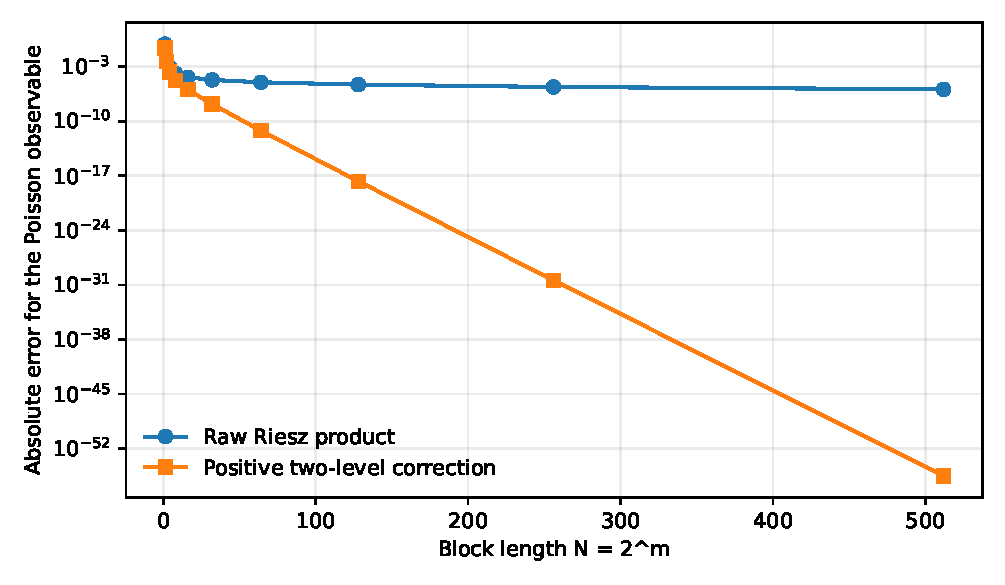
\includegraphics[width=0.94\textwidth]{figures/poisson_convergence.pdf}
\caption{The same Poisson errors. The raw error eventually follows $N^{-1}$;
the corrected error has the additional factor $(4/5)^N$. This dramatic gain is
for a fixed analytic observable, not a claim of total-variation convergence.}
\label{fig:poisson}
\end{figure}

\section{Exact dyadic energies and the classical moment exponent}
\label{sec:energy}

\subsection{A common two-dimensional transfer matrix}
The growth of $g(k)$ along powers of two alone does not determine its Sobolev
regularity. We need the total squared energy in a dyadic shell. Endpoint-weighted
sums eliminate otherwise distracting boundary terms. Define
\begin{align}
 U_m&=\sum_{k=1}^{N-1}g(k)^2+\frac12g(N)^2,&
 V_m&=\sum_{k=0}^{N-1}g(k)g(k+1),\label{eq:UV}\\
 X_m&=\sum_{k=1}^{N-1}\eta(k)^2+\frac59,&
 Y_m&=\sum_{k=0}^{N-1}\eta(k)\eta(k+1).
 \label{eq:XY}
\end{align}
The constant $5/9$ is the trapezoidal endpoint contribution
$(\eta(0)^2+\eta(N)^2)/2=(1+1/9)/2$.

\begin{proposition}[Exact energy recurrences]
\label{prop:energies}
Let
\begin{equation}
 M=\begin{pmatrix}6&2\\-4&-4\end{pmatrix}.
 \label{eq:M}
\end{equation}
Then
\begin{equation}
 \binom{U_{m+1}}{V_{m+1}}=M\binom{U_m}{V_m},\qquad
 \binom{X_{m+1}}{Y_{m+1}}=\frac14M\binom{X_m}{Y_m},
 \label{eq:energy-matrices}
\end{equation}
with $(U_0,V_0)=(1/2,0)$ and $(X_0,Y_0)=(5/9,-1/3)$.
\end{proposition}
\begin{proof}
For $g$, the even-index contribution to $U_{m+1}$ is $4U_m$, including the
half-weighted endpoint. The odd-index contribution is
\[
 \sum_{r=0}^{N-1}(g(r)+g(r+1))^2=2U_m+2V_m,
\]
because $g(0)=0$. Thus $U_{m+1}=6U_m+2V_m$. Adjacent pairs at the two parities
contribute
\[
 \sum_{r=0}^{N-1}\bigl[-2g(r)(g(r)+g(r+1))
       -2(g(r)+g(r+1))g(r+1)\bigr]
 =-4U_m-4V_m.
\]
This proves the first matrix equation.

For $\eta$, the even contribution to the trapezoidal square sum is $X_m$.
The odd contribution is $(2X_m+2Y_m)/4$, giving
$X_{m+1}=(3X_m+Y_m)/2$. The adjacent-pair sum is
$-(2X_m+2Y_m)/2=-X_m-Y_m$. This is precisely $M/4$.
The initial values follow from $N=1$, $g(1)=1$, and $\eta(1)=-1/3$.
\end{proof}

\begin{corollary}[Closed forms]
\label{cor:energy-closed}
Put $d=\sqrt{17}$, $\Lambda=1+d$, and $q=\Lambda/4$. Then
\begin{align}
 U_m&=\frac{5+d}{4d}\Lambda^m
      +\frac{d-5}{4d}(1-d)^m,\label{eq:U-closed}\\
 X_m&=\frac{19+5d}{18d}q^m
      +\frac{5d-19}{18d}\left(\frac{1-d}{4}\right)^m.
 \label{eq:X-closed}
\end{align}
In particular, $U_m\asymp\Lambda^m$ and $X_m\asymp q^m$.
\end{corollary}
\begin{proof}
The characteristic polynomial of $M$ is $t^2-2t-16$. Hence
$U_{m+2}=2U_{m+1}+16U_m$ with $U_0=1/2$, $U_1=3$.
For $M/4$ it is $t^2-t/2-1$, and $X_0=5/9$, $X_1=2/3$.
Solving these second-order recurrences gives the displayed formulas. The
coefficients of the dominant positive roots are positive and the other roots
have smaller modulus, proving the comparisons.
\end{proof}

For clarity about prior work, $\sum_{k=0}^{N-1}\eta(k)^2=X_m+4/9$ is the
square-correlation formula recorded in~\cite{CMPS}. It is not a new exponent
calculation. What matters here is that the boundary sequence has the \emph{same}
energy matrix, without the factor $1/4$.

\subsection{The fourth moment as a Stern energy}
\begin{proposition}
\label{prop:fourth}
For $N=2^m$,
\begin{equation}
 \int_0^1|P_m(\ee^{2\pi\ii x})|^4\dd x=2U_m,
 \qquad \norm{f_m}_{L^2}^2=\frac{2U_m}{N^2}.
 \label{eq:fourth}
\end{equation}
\end{proposition}
\begin{proof}
The coefficients of $P_m(z)^2$ through degree $N-1$ equal
$g(1),\ldots,g(N)$, since truncating $E$ at degree $N-1$ cannot change these
convolution coefficients. The reflection identity
$z^{N-1}P_m(z^{-1})=(-1)^mP_m(z)$ makes $P_m^2$ palindromic. Its coefficient
squares therefore sum to
$2\sum_{k=1}^{N-1}g(k)^2+g(N)^2=2U_m$. Parseval applied to $P_m^2$ proves the
first equation, and division by $N^2$ proves the second.
\end{proof}

This connects our transfer calculation to the classical even-moment setting
of~\cite{MMR}. It also avoids numerical integration of highly oscillatory products.

\subsection{Dyadic shell estimates}
Define
\begin{equation}
 \sigma=\frac12\log_2\frac{1+\sqrt{17}}4
       =0.178509318430288\ldots,\qquad
 s_* = 1+\sigma=1.178509318430288\ldots.
 \label{eq:exponents}
\end{equation}
The familiar correlation dimension is $D_2=1-2\sigma
=3-\log_2(1+\sqrt{17})$~\cite{ZPK}. We will use only the energy estimates,
not a new dimension theorem.

\begin{lemma}[Two-sided shell energies]
\label{lem:shell}
With $N=2^m$, constants independent of $m$ give
\begin{equation}
 \sum_{N<k\le2N}g(k)^2\asymp N^{2s_*},\qquad
 \sum_{N<k\le2N}\eta(k)^2\asymp N^{2\sigma}.
 \label{eq:shells}
\end{equation}
\end{lemma}
\begin{proof}
Let $G_m=\sum_{k=1}^Ng(k)^2=U_m+4^m/2$.
Then the first shell sum is
$G_{m+1}-G_m=U_{m+1}-U_m+3\cdot4^m/2$.
Since $\Lambda>4$ and the dominant coefficient in~\eqref{eq:U-closed} is
positive, this is a positive constant times $\Lambda^m$ asymptotically.
The remaining finitely many shells have positive energy, so constants can be
adjusted to cover them all. For $\eta$, the corresponding prefix sum through
$N$ is $X_m-4/9$. Its shell difference is $X_{m+1}-X_m$, asymptotic to a
positive constant times $q^m$, since $q>1$. Each shell contains a power of two,
where $\eta=-1/3$, so again every finite initial shell is nonzero. Finally
$\Lambda^m=N^{2s_*}$ and $q^m=N^{2\sigma}$.
\end{proof}

\section{Sharp Sobolev regularity and finite-size convergence}
\label{sec:sobolev}

\subsection{The function spaces and a shell-summation lemma}
For a periodic distribution $u$, use the norm
\begin{equation}
 \norm{u}_{H^{-s}}^2=
 \sum_{k\in\Z}(1+k^2)^{-s}|\widehat u(k)|^2.
 \label{eq:Sobolev}
\end{equation}
The use of $k$ rather than $2\pi k$ fixes constants but not thresholds. A pairing
with $\phi\in H^s$ is bounded by $\norm{u}_{H^{-s}}\norm{\phi}_{H^s}$.

\begin{lemma}[Weighted dyadic sums]
\label{lem:weighted}
Suppose $a_k\ge0$ and
$\sum_{2^j<k\le2^{j+1}}a_k\asymp2^{2tj}$, with a nonzero fixed low coefficient.
For $N=2^m$ and $s>t$,
\begin{equation}
 \sum_{k>N}(1+k^2)^{-s}a_k\asymp N^{2(t-s)}.
 \label{eq:weighted-tail}
\end{equation}
The full weighted series converges if and only if $s>t$. Moreover, for positive
$s$ the prefix sum through $N$ is, as $N\to\infty$,
\begin{equation}
 \sum_{1\le k\le N}(1+k^2)^{-s}a_k\asymp
 \begin{cases}
 N^{2(t-s)},&s<t,\\
 \log N,&s=t,\\
 1,&s>t.
 \end{cases}
 \label{eq:weighted-prefix}
\end{equation}
\end{lemma}
\begin{proof}
On the $j$th shell, the weight is comparable to $2^{-2sj}$, with comparison
constants depending only on $s$. The shell's weighted contribution is therefore
comparable to $2^{2(t-s)j}$. Summing this geometric progression over $j\ge m$
gives~\eqref{eq:weighted-tail}; convergence fails at equality because each shell
then contributes a positive amount. Summing over $j<m$ gives respectively a
last-term-dominated progression, $m$ comparable summands, or a bounded convergent
series. The nonzero low coefficient gives the last case's positive lower bound.
\end{proof}

\begin{theorem}[Exact regularity thresholds]
\label{thm:regularity}
The limiting measure and its boundary correction satisfy
\begin{equation}
 \mu\in H^{-s}\ \Longleftrightarrow\ s>\sigma,
 \qquad
 \nu\in H^{-s}\ \Longleftrightarrow\ s>s_*.
 \label{eq:regularity}
\end{equation}
Neither endpoint is included.
\end{theorem}
\begin{proof}
Apply Lemma~\ref{lem:weighted} to the two shell estimates in
Lemma~\ref{lem:shell}. Evenness duplicates the positive frequencies, and the
constant Fourier coefficient does not affect convergence. The factor $1/3$
in $\widehat\nu$ changes only the norm constant.
\end{proof}

The difference of exactly one in the thresholds expresses a genuine derivative's
worth of additional roughness in the universal correction. It is compatible with,
but substantially more precise than, the pointwise bound $|g(k)|\le k$.

\subsection{Norm convergence of the renormalized error}
\begin{theorem}[Sharp topology for the first correction]
\label{thm:renormalized}
Set $Z_m=(-1)^mN(\mu_m-\mu)$. Then
\begin{equation}
 Z_m\longrightarrow\nu\quad\hbox{in }H^{-s}
 \quad\Longleftrightarrow\quad s>s_*.
 \label{eq:Z-limit}
\end{equation}
For $s>s_*$,
\begin{equation}
 \norm{Z_m-\nu}_{H^{-s}}\ll_s N^{s_*-s}.
 \label{eq:Z-rate}
\end{equation}
\end{theorem}
\begin{proof}
On $|k|\le N$ the difference vanishes. On the complement it equals
$-(-1)^mN\eta(|k|)-g(|k|)/3$. The squared norm is bounded by a fixed constant
times the sum of $N^2$ times the $\eta$ tail energy and the $g$ tail energy.
By~\eqref{eq:weighted-tail}, both have size at most $N^{2(s_*-s)}$.
This proves the norm bound and convergence. Conversely, a norm limit in
$H^{-s}$ must have every Fourier coefficient equal to the eventually exact
coefficient $g(|k|)/3$, hence must be $\nu$. That distribution belongs to
$H^{-s}$ only for $s>s_*$. For $s\le\sigma$, already $\mu_m-\mu$ is not an
element of $H^{-s}$; the finite polynomial cannot remove the divergent tail.
\end{proof}

\subsection{The raw approximation: a phase transition and saturation}
\begin{theorem}[Sharp raw error rates]
\label{thm:raw-rate}
For every fixed $s>\sigma$, as $N=2^m\to\infty$,
\begin{equation}
 \boxed{\quad
 \norm{\mu_m-\mu}_{H^{-s}}\asymp_s
 \begin{cases}
 N^{\sigma-s},&\sigma<s<s_*,\\
 N^{-1}\sqrt{\log N},&s=s_*,\\
 N^{-1},&s>s_*.
 \end{cases}\quad}
 \label{eq:raw-rates}
\end{equation}
For $s>s_*$ there is also the exact leading norm limit
\begin{equation}
 N\norm{\mu_m-\mu}_{H^{-s}}\longrightarrow\norm{\nu}_{H^{-s}}>0.
 \label{eq:raw-leading-norm}
\end{equation}
\end{theorem}
\begin{proof}
Because the finite coefficients vanish beyond their support, the squared norm
has the exact decomposition
\begin{equation}
 \norm{\mu_m-\mu}_{H^{-s}}^2
 =\frac{2}{9N^2}\sum_{k=1}^{N}(1+k^2)^{-s}g(k)^2
   +2\sum_{k>N}(1+k^2)^{-s}\eta(k)^2.
 \label{eq:exact-norm-decomposition}
\end{equation}
The endpoint $k=N$ is included in the first sum by Theorem~\ref{thm:boundary}.
Use~\eqref{eq:weighted-prefix} with $t=s_*$ for the first term and
\eqref{eq:weighted-tail} with $t=\sigma$ for the second. If $s<s_*$, both are
of order $N^{2(\sigma-s)}$. At $s=s_*$ the first is of order
$N^{-2}\log N$, while the second is of order $N^{-2}$. Above $s_*$ the first
is of order $N^{-2}$ and the second is smaller. Taking square roots proves the
three regimes. Equation~\eqref{eq:raw-leading-norm} follows from
Theorem~\ref{thm:renormalized} and continuity of the norm; $\nu\ne0$ because
its first coefficient is $1/3$.
\end{proof}

Thus additional smoothness ceases to improve the raw rate after $s_*$. The
obstruction is not an estimate artifact: it is a specific nonzero distribution,
with an exactly known Fourier series.

\subsection{The corrected approximation removes saturation}
\begin{theorem}[Sharp corrected rate and bandwidth optimality]
\label{thm:corrected-rate}
For every fixed $s>\sigma$,
\begin{equation}
 \boxed{\quad
 \norm{\mt_m-\mu}_{H^{-s}}\asymp_s N^{\sigma-s}.
 \quad}
 \label{eq:corrected-rates}
\end{equation}
More generally, fix $C>0$. Every approximant $v_N$ whose Fourier support is
contained in $|k|\le CN$ satisfies, for all sufficiently large dyadic $N$,
\begin{equation}
 \norm{v_N-\mu}_{H^{-s}}\ge c_{s,C}N^{\sigma-s}.
 \label{eq:bandwidth-lower}
\end{equation}
No positivity assumption on $v_N$ is required for this lower bound.
\end{theorem}
\begin{proof}
The corrected error vanishes through $N$. For the middle band $N<|k|<2N$,
use $(1+k^2)^{-s}\le N^{-2s}$ and
$|a-b|^2\le2|a|^2+2|b|^2$. By~\eqref{eq:positive-density} and Parseval,
\[
 \sum_k|\widehat{\mt_m}(k)|^2
 =\norm{\ft_m}_{L^2}^2
 \le\frac{25}{9}\norm{f_m}_{L^2}^2
 =\frac{50U_m}{9N^2}\ll N^{2\sigma}.
\]
The $\eta$ energy on the middle band has the same upper order by
Lemma~\ref{lem:shell}. Thus that band's weighted contribution is
$O_s(N^{2(\sigma-s)})$. Beyond $2N$ the approximant has no coefficients, and
Lemma~\ref{lem:weighted} gives the same order for the tail. This proves the
upper bound. The unchanged $\eta$ tail beyond $2N$ alone proves the matching
lower bound.

For the general assertion, choose a fixed integer $j$ with $2^j>C$ and take the
shell $2^jN<|k|\le2^{j+1}N$. All coefficients of $v_N$ there vanish. Its
weighted $\eta$ energy is bounded below by a constant times
$N^{2(\sigma-s)}$. Taking a square root proves~\eqref{eq:bandwidth-lower}.
\end{proof}

For rough admissible tests, $\sigma<s<s_*$, the correction improves the constant
and exactness band but cannot improve the order dictated by the unresolved
spectral tail. At the threshold it removes $\sqrt{\log N}$, and above the
threshold it removes the $N^{-1}$ saturation completely. These are different
regimes of a single exact identity, rather than competing convergence claims.

\section{A parameter family and the sharp positivity threshold}
\label{sec:parameter}

\subsection{Amplitude-deformed binary Riesz products}
For $-1\le a\le1$, define
\begin{equation}
 f_m^{(a)}(x)=\prod_{j=0}^{m-1}(1-a\cos(2\pi2^jx)),\qquad
 \mu_m^{(a)}=f_m^{(a)}(x)\dd x.
 \label{eq:parameter-product}
\end{equation}
These are amplitude deformations; no identification with a differently
parameterized phase-deformation family is intended. Every factor is nonnegative.
The constant coefficient remains one: in
$f_{m+1}^{(a)}=(1-a\cos(2\pi x))f_m^{(a)}(2x)$, the last factor has only even
frequencies. Hence all $\mu_m^{(a)}$ are probabilities. Their Fourier recursion is
\begin{equation}
 r_{m+1}^{(a)}(2r)=r_m^{(a)}(r),\qquad
 r_{m+1}^{(a)}(2r+1)=-\frac a2\bigl(r_m^{(a)}(r)+r_m^{(a)}(r+1)\bigr).
 \label{eq:parameter-rec}
\end{equation}
The same fixed-index induction as in Proposition~\ref{prop:limit} proves a weak
limit $\mu^{(a)}$, whose coefficients $\eta_a$ obey this recursion with
\begin{equation}
 \eta_a(0)=1,\qquad \eta_a(1)=-\frac a{2+a}.
 \label{eq:parameter-eta}
\end{equation}
The coefficient bound $|\eta_a(k)|\le1$ follows from the probability measure.

When $a=0$, every measure is Lebesgue measure. When $a=1$, we recover the
Thue--Morse case. At $a=-1$,
\begin{equation}
 f_m^{(-1)}(x)=\frac1N\left|\sum_{n=0}^{N-1}\ee^{2\pi\ii nx}\right|^2,
 \label{eq:Fejer}
\end{equation}
the dyadic Fej\'er kernel; its coefficients tend to one, so its limit is the point
mass at zero. This endpoint is a useful exact check on the general formulas.

\begin{theorem}[Parameterized Stern boundary]
\label{thm:parameter-boundary}
Fix $a\in[-1,1]\setminus\{0\}$, and write
\begin{equation}
 \alpha=-\frac a2,\qquad c=\frac a{2+a},\qquad
 g_a(k)=B_k(-2/a).
 \label{eq:parameter-g}
\end{equation}
Then, exactly for $0\le k\le N=2^m$,
\begin{equation}
 r_m^{(a)}(k)-\eta_a(k)=c\alpha^m g_a(k).
 \label{eq:parameter-boundary}
\end{equation}
\end{theorem}
\begin{proof}
The initial coefficient at $k=1$ has error $c$, agreeing with $g_a(1)=1$.
The even recursion for $g_a$ multiplies by $-2/a=\alpha^{-1}$, compensating for
the extra $\alpha$ at the next level. Its odd recursion is the sum of two
adjacent values, exactly matching the factor $\alpha$ in the Fourier recursion.
The induction of Theorem~\ref{thm:boundary}, with these constants substituted,
therefore proves the statement, including the endpoint.
\end{proof}

\begin{theorem}[Exactness and a sharp positivity interval]
\label{thm:parameter-positive}
For $a\in[-1,1]$, put
\begin{equation}
 \mt_m^{(a)}=\frac{a\mu_m^{(a)}+2\mu_{m+1}^{(a)}}{2+a}.
 \label{eq:parameter-correction}
\end{equation}
It has total mass one and agrees with $\mu^{(a)}$ at every Fourier mode
$|k|\le N$. Its density is
\begin{equation}
 \ft_m^{(a)}(x)=f_m^{(a)}(x)
     \left(1-\frac{2a}{2+a}\cos(2\pi Nx)\right).
 \label{eq:parameter-density}
\end{equation}
For every $m$, this density is nonnegative on the whole circle if and only if
\begin{equation}
 \boxed{\qquad -\frac23\le a\le1.\qquad}
 \label{eq:positivity-threshold}
\end{equation}
For $a\ne0$, the affine combination is uniquely determined by exactness at the
first mode. At $a=0$ all levels coincide and uniqueness is not asserted.
\end{theorem}
\begin{proof}
For $a\ne0$, the common-band errors have ratio $\alpha=-a/2$. Their cancellation
condition is $w+(1-w)\alpha=0$, giving $w=a/(2+a)$. The density identity follows
by factoring $f_{m+1}^{(a)}=f_m^{(a)}(1-a\cos(2\pi Nx))$. The second factor is
nonnegative exactly when $|2a/(2+a)|\le1$, which on $[-1,1]$ is $a\ge-2/3$.
This condition is sufficient since $f_m^{(a)}\ge0$. If $a<-2/3$, the second
factor is negative where $\cos(2\pi Nx)=-1$, for example at $x=1/(2N)$:
its value there is $(2+3a)/(2+a)<0$. Every factor of $f_m^{(a)}$ at this point
is strictly positive, since for $j<m$,
$0<2\pi2^jx\le\pi/2$ and $1-a\cos(2\pi2^jx)\ge1$.
Thus the corrected density is strictly negative on a neighborhood of this point.
This proves necessity,
including the endpoint $a=-1$. The case $a=0$ is immediate.
\end{proof}

\begin{remark}[Negative weights need not force a negative density]
For $-2/3\le a<0$, the coefficient of $\mu_m^{(a)}$ in the affine combination
is negative, yet the resulting density is nonnegative. The factorization, rather
than the signs of the mixing weights alone, decides positivity. Below $-2/3$
this exact two-level construction genuinely becomes signed. The theorem is a
sharp threshold for this construction, not a no-go theorem for every possible
positive approximation with a larger number of levels.
\end{remark}

\subsection{The full fixed-parameter Sobolev rate law}
The same mechanism has a continuous family of exponents. The proof is included
because the amplitude deformation separates two roles that coincide at $a=1$:
the boundary's geometric decay factor and the limiting measure's energy growth.
Set
\begin{align}
 T_a&=1-a+\frac{a^2}{2},&
 \rho_a&=\frac{T_a+\sqrt{T_a^2+4a}}2,\label{eq:rhoa}\\
 \beta_a&=\log_2\frac2{|a|},&
 \sigma_a&=\frac12\log_2\rho_a,& s_a&=\sigma_a+\beta_a.
 \label{eq:param-exponents}
\end{align}
These quantities are defined for fixed $a\ne0$ in $[-1,1]$.

\begin{theorem}[Parameterized regularity and sharp rates]
\label{thm:parameter-rates}
Let $\widehat\nu_a(0)=0$ and
$\widehat\nu_a(k)=c\,g_a(|k|)$ for $k\ne0$, with $c$ as
in~\eqref{eq:parameter-g}. Then
\begin{equation}
 \mu^{(a)}\in H^{-s}\ \Longleftrightarrow\ s>\sigma_a,
 \qquad \nu_a\in H^{-s}\ \Longleftrightarrow\ s>s_a.
 \label{eq:param-reg}
\end{equation}
For every fixed $s>\sigma_a$,
\begin{align}
 \norm{\mu_m^{(a)}-\mu^{(a)}}_{H^{-s}}
 &\asymp_{a,s}
 \begin{cases}
 N^{\sigma_a-s},&\sigma_a<s<s_a,\\
 N^{-\beta_a}\sqrt{\log N},&s=s_a,\\
 N^{-\beta_a},&s>s_a,
 \end{cases}\label{eq:param-raw}\\
 \norm{\mt_m^{(a)}-\mu^{(a)}}_{H^{-s}}
 &\asymp_{a,s}N^{\sigma_a-s}.
 \label{eq:param-corrected}
\end{align}
The corrected estimate remains valid below the positivity threshold, where the
approximants are signed. For $s>s_a$, the renormalized errors converge to
$\nu_a$ in $H^{-s}$ after multiplication by $\alpha^{-m}$, with error
$O_{a,s}(N^{s_a-s})$.
\end{theorem}
\begin{proof}
Put $b=-2/a$ and define trapezoidal energies
\begin{align*}
 U_m^{(a)}&=\sum_{k=1}^{N-1}g_a(k)^2+\tfrac12g_a(N)^2,&
 V_m^{(a)}&=\sum_{k=0}^{N-1}g_a(k)g_a(k+1),\\
 X_m^{(a)}&=\sum_{k=1}^{N-1}\eta_a(k)^2+\tfrac12(1+c^2),&
 Y_m^{(a)}&=\sum_{k=0}^{N-1}\eta_a(k)\eta_a(k+1).
\end{align*}
The same even-odd splitting used in Proposition~\ref{prop:energies} gives
\begin{equation}
 \binom{X_{m+1}^{(a)}}{Y_{m+1}^{(a)}}=
 M_a\binom{X_m^{(a)}}{Y_m^{(a)}},\qquad
 M_a=\begin{pmatrix}1+a^2/2&a^2/2\\-a&-a\end{pmatrix},
 \label{eq:param-energy}
\end{equation}
and
\begin{equation}
 \binom{U_{m+1}^{(a)}}{V_{m+1}^{(a)}}=
 \begin{pmatrix}b^2+2&2\\2b&2b\end{pmatrix}
 \binom{U_m^{(a)}}{V_m^{(a)}}
 =\frac4{a^2}M_a\binom{U_m^{(a)}}{V_m^{(a)}}.
 \label{eq:param-genergy}
\end{equation}
For example the odd square contribution for $g_a$ is $2U_m^{(a)}+2V_m^{(a)}$;
the adjacent-pair sum is $2b(U_m^{(a)}+V_m^{(a)})$. For $\eta_a$, the odd square
contribution is $a^2(X_m^{(a)}+Y_m^{(a)})/2$, and the adjacent-pair sum is
$-a(X_m^{(a)}+Y_m^{(a)})$. These establish both matrices without omitted
boundary terms.

The characteristic polynomial of $M_a$ is $x^2-T_ax-a$. Its discriminant is
positive. For $a\ge0$ this is immediate. For $a=-u<0$ it is
$(1-u)^2+u^2+u^3+u^4/4>0$. Evaluating the polynomial at one gives $-a^2/2<0$,
so the larger root $\rho_a$ exceeds one. The other root has modulus
$|a|/\rho_a<1$. Thus each first-coordinate energy is a combination of two
distinct real geometric sequences. The coefficient of $\rho_a^m$ in
$X_m^{(a)}$ is strictly positive: otherwise nonnegativity rules out a negative
coefficient, while a zero coefficient would make the energy bounded, contrary
to the $m$ nonzero values $\eta_a(2^j)=-c$ in its prefix.
For $U_m^{(a)}$, the larger eigenvalue is $(4/a^2)\rho_a>b^2$. The coefficient
of that root is again positive: a zero dominant coefficient would contradict
$U_m^{(a)}\ge b^{2m}/2$, because the smaller root has modulus strictly less than
$b^2$.

Consequently, taking differences of prefix energies as in
Lemma~\ref{lem:shell},
\[
 \sum_{N<k\le2N}\eta_a(k)^2\asymp_a N^{2\sigma_a},\qquad
 \sum_{N<k\le2N}g_a(k)^2\asymp_a N^{2s_a}.
\]
The endpoints $g_a(N)^2=b^{2m}$ are lower order than the dominant energy;
the endpoints $\eta_a(N)^2=c^2$ are constant. All finite shells have positive
energy because they contain powers of two. The sequence $g_a$ also has
polynomial growth: $|g_a(k)|\le k^{\beta_a}$ follows by induction from
$|b|=2^{\beta_a}$ and
$r^{\beta_a}+(r+1)^{\beta_a}\le(2r+1)^{\beta_a}$, since $\beta_a\ge1$.
Thus $\nu_a$ is a distribution.

The shell-summation lemma now proves~\eqref{eq:param-reg}. On the low band the
raw error is exactly $c\alpha^mg_a(k)$, with
$|\alpha|^m=N^{-\beta_a}$; outside the support it is $-\eta_a(k)$. Applying
the weighted prefix and tail estimates gives~\eqref{eq:param-raw}, including
the logarithm at the critical exponent. The same tail argument proves the
renormalized convergence and its rate.

For the corrected upper bound, its support is contained in $|k|<2N$ and its
error vanishes through $N$. The low-band identity also gives
\[
 \sum_k|r_m^{(a)}(k)|^2
 \ll_a \sum_{k=0}^{N}\eta_a(k)^2+
        |\alpha|^{2m}\sum_{k=0}^{N}g_a(k)^2
 \ll_a N^{2\sigma_a}.
\]
The multiplicative factor in~\eqref{eq:parameter-density} is bounded in absolute
value by $1+2|a|/(2+a)$. Hence its corrected $L^2$ norm has the same upper order,
even when the factor changes sign. Bounding the middle band and the untouched
tail exactly as in Theorem~\ref{thm:corrected-rate} proves the upper bound in
\eqref{eq:param-corrected}. The tail beyond $2N$ proves the lower bound.
\end{proof}

At $a=-1$, the formulas give $\rho_a=2$, $\sigma_a=1/2$, $\beta_a=1$, and
$s_a=3/2$. Also $g_a(k)=B_k(2)=k$ and $c=-1$, so
$r_m^{(-1)}(k)=1-k/N$ on $0\le k\le N$, the familiar Fej\'er coefficients.
At $a=1$, every formula reduces to the Thue--Morse theorem. The limit $a\to0$
is not uniform in the constants: the case $a=0$ is exactly constant in $m$ and
is correctly excluded from the exponent parametrization.

\section{Computation, verification, and proof engineering}
\label{sec:computation}

\subsection{Exact computation without constructing a large block}
To compute a single stabilized finite Fourier coefficient, choose $m$ with
$2^m\ge k$, compute $\eta(k)$ from its two adjacent-value recursion, compute
$g(k)$ using~\eqref{eq:binary-matrices}, and apply~\eqref{eq:main-boundary}.
The state for $\eta$ has matrices
\begin{equation}
 \binom{\eta(2k)}{\eta(2k+1)}=
 \begin{pmatrix}1&0\\-1/2&-1/2\end{pmatrix}
 \binom{\eta(k)}{\eta(k+1)},\qquad
 \binom{\eta(2k+1)}{\eta(2k+2)}=
 \begin{pmatrix}-1/2&-1/2\\0&1\end{pmatrix}
 \binom{\eta(k)}{\eta(k+1)}.
 \label{eq:eta-binary-matrices}
\end{equation}
Starting from $(\eta(0),\eta(1))=(1,-1/3)$ and reading the bits from most to
least significant takes $O(\log k)$ arithmetic operations. Leading zero bits
leave this initial state unchanged. These are arithmetic-operation counts;
bit complexity also accounts for integer sizes. The signed Stern values have
$O(\log k)$ bits by $|g(k)|\le k$, and the rational recursion for $\eta$ grows
its denominator by at most one factor of two per bit.

When all coefficients through $N$ are required, the descending recurrences can
be tabulated in $O(N)$ arithmetic operations and memory. Directly summing all
correlations takes $O(N^2)$ sign multiplications; an FFT is an alternative for
approximation, but the recurrence plus exact boundary term provides exact
rational coefficients without rounding.

For the analytic correction, the finite formula~\eqref{eq:kappa-finite} uses only
$1+\vnu(n)$ binary partition values. A table of $p_2(0),\ldots,p_2(L)$ can be
computed by a coin-change dynamic program, using two colors of each size
$1,2,4,\ldots$, in $O(L\log L)$ integer additions. Formula~\eqref{eq:K-Mahler}
then computes all $\kappa_n$ in $O(L)$ rational operations. Positivity prevents
large cancellation when evaluating $K(t)$ for real $0<t<1$.

\subsection{Avoiding loss of the corrected error}
At large $N$, directly subtracting two nearly equal high-precision expectations
can lose most significant digits. Equation~\eqref{eq:corrected-poisson} is a
better evaluation formula. Even within that formula, write
\begin{equation}
 K(t)-K(t^2)=\sum_{j\ge1}\kappa_jt^j(1-t^j),\qquad 0<t<1,
 \label{eq:positive-evaluation}
\end{equation}
instead of subtracting two numbers close to one. Every summand is positive.
For very small $t$, one can factor out $3t$ before accumulating the remaining
series. For complex $z$ or shifted observables this particular positivity is
lost, but the exact disk factorization still applies.

\subsection{The supplied verification program}
The companion \texttt{verify.py} uses only Python's standard library. Identity
checks use integers and \texttt{fractions.Fraction}; none uses floating-point
equality. The recorded run performs 19,037 checks, including:
\begin{center}
\begin{tabularx}{\textwidth}{@{}p{0.39\textwidth}X@{}}
\toprule
Test family & Range or independent representation \\
\midrule
Aperiodic and forward corrections & Every $0\le k\le2^m$ for $0\le m\le10$. \\
Finite Fourier products & Independent Laurent-polynomial multiplication of all factors. \\
Positive correction and first missed mode & Exact low-band agreement and the coefficient at $N+1$. \\
Signed Stern identity & Direct sign convolution through $k=1024$, bounds, and valuations. \\
Energy transfer and fourth moments & Exact rational sums through level $12$. \\
Analytic factorization & Every coefficient through degree $256$ at levels $0$ through $7$. \\
Partition coefficient formula & Exact coefficients, finite sums, and positivity bounds through $256$. \\
Amplitude family & Nine nonzero rational parameters, every low mode through level $7$, and both energy matrices. \\
\bottomrule
\end{tabularx}
\end{center}
The parameters are $-1,-3/4,-2/3,-1/2,-1/7,1/7,1/4,1/2,1$.
These tests are not replacements for proofs of infinite statements. They check
independent finite representations and are particularly effective at catching
endpoint, sign, normalization, and parameter mistakes.

\texttt{make\_figures.py} separately uses \texttt{mpmath}, \texttt{numpy}, and
\texttt{matplotlib}. The Poisson table uses 160 decimal digits and 2,201 terms
for its independent limiting-series evaluation. The data and the exact test
report are included as JSON. The verification program itself has no dependency
on those optional plotting packages.

\subsection{Formalization targets in the supplied repository}
No Lean source is supplied or claimed checked here. The following dependency
order isolates relatively small formal targets compatible with the atlas's
existing finite autocorrelation and polynomial-product development.

The first layer is entirely algebraic: define the convolution sequence $g$, prove
its two parity recurrences, identify it with $B_k(-2)$ if a Stern-polynomial
interface is desired, and prove the two exact boundary formulas. The latter
need only natural-number induction, finite sums, binary reflection, and rational
arithmetic. The central low-band cancellation is then a short consequence.

The second layer packages Fourier coefficients of finite trigonometric products.
Positivity of the corrected density is a direct bound on cosine, not a limiting
argument. Weak existence of $\mu$ can be taken from the existing development or
proved from finite coefficient convergence and compactness.

The third layer separates analysis from combinatorics: prove the two energy
matrix identities as finite-sum theorems, solve the scalar recurrences, derive
shell estimates, and then apply an abstract weighted-shell lemma. The sharp
Sobolev thresholds and all three error regimes become applications of that one
lemma to an exact norm decomposition. The analytic factorization is a separate
Mahler-equation branch; its only infinite-product requirements are local uniform
convergence and nonvanishing in the open disk.

This architecture deliberately avoids equating ``proved on paper'' with
``already formalized in the current repository.'' It also keeps classical
spectral-type results out of the dependencies of the new algebraic identities.

\section{Further questions suggested by the exact mechanism}
\label{sec:questions}

\subsection{Non-dyadic windows and binary boundary states}
For a length $L$ that is not a power of two, the finite word decomposes into
signed dyadic blocks. The single correction $g(k)$ should then be replaced by
several cross-boundary states whose coefficients depend on the binary expansion
of $L$. A concrete next problem is to derive a finite-dimensional exact state
system for these defects and determine which subsequences of $L$ admit positive
moment-exact combinations. The present theorems prove the one-state collapse
on dyadic lengths; they do not assert such a collapse for all lengths.

\subsection{Positive corrections for other substitution spectra}
The general principle is an affine finite Fourier recursion with a contractive
boundary eigenvalue. A negative eigenvalue allows cancellation by positive
weights on two consecutive levels, as in the Thue--Morse case. With several
boundary eigenvalues, the cancellation conditions become a finite moment problem
for the level weights. Determining when these weights, or the resulting density
factor, remain nonnegative is a concrete algebraic question. The interval
$[-2/3,1]$ in the amplitude family shows why positivity of the final factor can
be a less restrictive condition than positivity of every weight.

\subsection{Distribution functions and nonsmooth local probes}
Theorems~\ref{thm:raw-rate} and~\ref{thm:corrected-rate} describe an entire
Sobolev scale, but they do not automatically settle optimal uniform error for
cumulative distribution functions. Indicator functions are substantially less
smooth than the observables for which the first correction gives a full weak
expansion. A next step is to combine the exact band cancellation with sharp
local mass bounds for the Thue--Morse measure. This requires additional local
information, not another manipulation of the same fixed-mode identity.

\subsection{More layers versus more exact modes}
Two consecutive products uniquely cancel the one low-band boundary mode.
Three or more levels can cancel selected later analytic sectors in
\eqref{eq:lacunary-expansion}, but the variables at consecutive levels are
$z^N,z^{2N},z^{4N},\ldots$, not ordinary powers of a common mesh parameter.
A useful precise problem is to maximize the exact Fourier band subject to
nonnegative level weights, or more generally a nonnegative factored density.
The first missed coefficient~\eqref{eq:first-missed} supplies the first
nontrivial constraint. No general optimal multi-level scheme is claimed here.

\section{Conclusion}
The finite Thue--Morse diffraction defect is controlled by a simple object that
is invisible in a statement of weak convergence alone: the signed Stern sequence
$B_k(-2)$, equivalently the coefficients of $zE(z)^2$. On the full band
$0\le k\le2^m$, it gives an exact, alternating boundary term. This one identity
simultaneously explains the raw $N^{-1}$ saturation for smooth tests, produces a
positive Fourier-exact correction, and yields a universal rough distribution
whose Sobolev threshold is determined by a classical moment eigenvalue.

The analytic factorization goes beyond the low band. It expresses every remaining
finite-size sector through a single positive-coefficient function $K$, with explicit
finite formulas in two-colored binary partition numbers. For Poisson observables
this yields signed bounds and an exponential gain. The amplitude extension shows
which parts of the mechanism persist away from Thue--Morse and precisely where
positivity fails for the two-level construction. The resulting package is a
self-contained extension of the supplied atlas, with proved formulas, sharp
norm estimates, and reproducible exact checks rather than a list of numerical
conjectures.

\appendix
\section{Compact formula sheet}
\label{app:formula}
With $N=2^m$, $g(k)=B_k(-2)$, and $Q(z)=zE(z)^2$, the central formulas are
\begin{align*}
 r_m(k)-\eta(k)&=\frac{(-1)^m}{3N}g(k),&&0\le k\le N,\\
 A_m(k)-N\eta(k)&=-\frac23(-1)^mg(k),&&0\le k\le N,\\
 \mt_m&=(\mu_m+2\mu_{m+1})/3,&
 \ft_m&=f_m(1-\tfrac23\cos(2\pi Nx)),\\
 \widehat{\mt_m}(k)&=\eta(k),&&|k|\le N,\\
 \widehat\nu(k)&=g(|k|)/3,&&k\ne0,\\
 H_m-H&=\frac{(-1)^m}{3N}Q(z)K(z^N),&&|z|<1,\\
 2K(z)+K(z^2)&=3E(z)^{-2},&K(0)&=1,\\
 \kappa_n&=\frac32\sum_{j=0}^{\vnu(n)}(-1/2)^jp_2(n/2^j),&&n\ge1.
\end{align*}
The exponents are
\[
 \sigma=\frac12\log_2\frac{1+\sqrt{17}}4,\qquad s_*=1+\sigma.
\]
The raw Sobolev rate is $N^{\sigma-s}$ below $s_*$, $N^{-1}\sqrt{\log N}$ at
$s_*$, and $N^{-1}$ above it. The corrected rate is $N^{\sigma-s}$ throughout
$s>\sigma$. Every use of these rates fixes $s$ before taking $N\to\infty$.

\section{Reproduction commands and file manifest}
\label{app:reproduction}
Run the exact checks independently of the document build:
\begin{lstlisting}
python verify.py --output verification.json
\end{lstlisting}
The included report uses the default maximum direct-correlation level $10$.
A larger finite test can be requested with \texttt{--max-level 11}; direct
correlation tests have quadratic cost in block length. Python 3.9 or later is
sufficient for this standard-library program.

The figures and high-precision table are already included. To regenerate them,
install the optional dependencies and run:
\begin{lstlisting}
python -m pip install numpy matplotlib mpmath
python make_figures.py
\end{lstlisting}
The article uses a single main \texttt{.tex} file with an inline bibliography,
a small generated table, and two figure PDFs. Build with a conventional TeX Live
installation:
\begin{lstlisting}
latexmk -pdf -interaction=nonstopmode -halt-on-error \
  Thue_Morse_Boundary_Corrections.tex
\end{lstlisting}
The preamble uses Libertinus when installed and falls back to Latin Modern.
No font files are distributed. The ZIP includes the compiled article, its sources,
the two reproducibility scripts, JSON data, rendered figure files, and a README.

\begin{thebibliography}{9}
\addcontentsline{toc}{section}{References}

\bibitem{atlas}
Vladimir Reshetnikov's \texttt{ProveIt} repository,
\emph{The Thue--Morse Sequence: Formula Atlas and Fabius--Rvachev Frontier Results},
consolidated document dated 28 August 2026; retrieved 4 September 2026.
\url{https://github.com/VladimirReshetnikov/ProveIt/tree/main/Analysis/FabiusFunction/docs/semi-formalized-research-frontiers/drafts/thue-morse/Thue_Morse_Atlas_and_Frontiers}.
The inspected source blob is recorded in Section~\ref{sec:scope}.

\bibitem{BG}
Michael Baake and Uwe Grimm,
\emph{The singular continuous diffraction measure of the Thue--Morse chain},
Journal of Physics A: Mathematical and Theoretical \textbf{41} (2008), 422001.
\href{https://doi.org/10.1088/1751-8113/41/42/422001}{doi:10.1088/1751-8113/41/42/422001}.
Open manuscript: \url{https://arxiv.org/abs/0809.0580}.

\bibitem{Stern}
Sandi Klav\v zar, Uro\v s Milutinovi\'c, and Ciril Petr,
\emph{Stern polynomials},
Advances in Applied Mathematics \textbf{39} (2007), no.~1, 86--95.
\href{https://doi.org/10.1016/j.aam.2006.01.003}{doi:10.1016/j.aam.2006.01.003}.

\bibitem{ZPK}
Michael A. Zaks, Arkady S. Pikovsky, and J\"urgen Kurths,
\emph{On the correlation dimension of the spectral measure for the Thue--Morse sequence},
Journal of Statistical Physics \textbf{88} (1997), 1387--1392.
\href{https://doi.org/10.1007/BF02732440}{doi:10.1007/BF02732440}.

\bibitem{MMR}
Christian Mauduit, Hugh L. Montgomery, and Jo\"el Rivat,
\emph{Moments of a Thue--Morse generating function},
Journal d'Analyse Math\'ematique \textbf{135} (2018), 713--724.
\href{https://doi.org/10.1007/s11854-018-0050-y}{doi:10.1007/s11854-018-0050-y}.

\bibitem{CMPS}
Michael Coons, Jan Maz\'a\v c, Ari Pincus--Kazmar, and Adam Stout,
\emph{On the absolute value of the autocorrelations of the Thue--Morse sequence},
Experimental Mathematics, published online 31 January 2026.
\href{https://doi.org/10.1080/10586458.2025.2602541}{doi:10.1080/10586458.2025.2602541}.
Open manuscript: \url{https://arxiv.org/abs/2511.06386}.
The explicit square-correlation formula is used only as acknowledged background;
the needed identity is rederived in Section~\ref{sec:energy}.

\bibitem{BC}
Michael Baake and Michael Coons,
\emph{Correlations of the Thue--Morse sequence},
Indagationes Mathematicae \textbf{35} (2024), no.~5, 914--930.
\href{https://doi.org/10.1016/j.indag.2023.02.001}{doi:10.1016/j.indag.2023.02.001}.
Open manuscript: \url{https://arxiv.org/abs/2209.07102}.

\end{thebibliography}
\end{document}
